\documentclass[handout, c,english]{beamer}
\usetheme{Frankfurt}
\usepackage[utf8]{inputenc}
\usepackage{natbib}
%\usepackage[french]{babel}
\usepackage[english]{babel}
\usepackage{listings}
\usepackage{hyperref}
\usepackage{tikz}
\usepackage{algorithm}
\usepackage[noend]{algpseudocode}
\usepackage{pgfplots}
\usepackage{comment}
\usepackage{todonotes}

%animations (for gifs)
\usepackage{animate}

%for figures
\usepackage{tikz}
\usetikzlibrary{positioning,calc,intersections, shapes.geometric, fit, backgrounds}

%used to plot results
\usepackage{pgfplots}
\usepackage{pgfplotstable}


%for subfigures
\usepackage{caption}
\usepackage{subcaption}
\usepackage{amssymb}

\setbeamertemplate{footline}[frame number]


\title{IEEE ICTAI 2022}
\subtitle{Extending a Refinement Acting Engine for Fleet Management: Concurrency and Resources}
\author{Jérémy Turi, Arthur Bit-Monnot \\
jeremy.turi@laas.fr, abitmonnot@laas.fr}
\institute{\textit{LAAS-CNRS, Université de Toulouse, CNRS, INSA,} Toulouse, France}
\date{\today}

\begin{document}

\begin{frame}
\titlepage
\end{frame}

\begin{frame}
\frametitle{Outline}
\tableofcontents
\end{frame}

\AtBeginSection[]
{
  \begin{frame}
    \frametitle{Table of Contents}
    \tableofcontents[currentsection]
  \end{frame}
}

\section{Introduction}
\subsection{Deliberation for logistic}

\begin{frame}{Industry 4.0: Logistic enhanced by robotics}
    \centering
\begin{columns}
    \begin{column}{0.5\textwidth}
        Improve flexibility and efficiency of factories using a fleet of Autonomous Mobile Robots (AMRs):
        \begin{itemize}
            \pause
            \item Automate task allocation to AMR
            \pause
            \item Deal with contingencies and deadlines
            \pause
            \item Optimize the overall process in functio of time, energy, etc.
        \end{itemize}
    \end{column}
    \begin{column}{0.5\textwidth}
        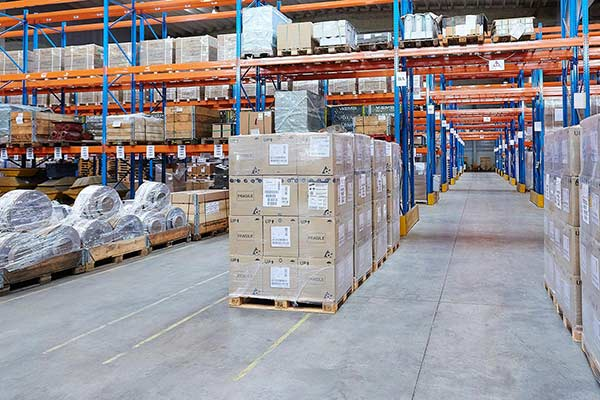
\includegraphics[width = \textwidth]{images/logisticsolutions.jpg}
    \end{column}
\end{columns}
\end{frame}

\begin{frame}{GobotSim, a new factory simulator with an emphasis on deliberation}
    \begin{columns}
        \begin{column}{0.5\textwidth}
            GobotSim, a 2D factory simulator to study scheduling and resource allocation strategies.
        \end{column}
        \begin{column}{0.4\textwidth}
            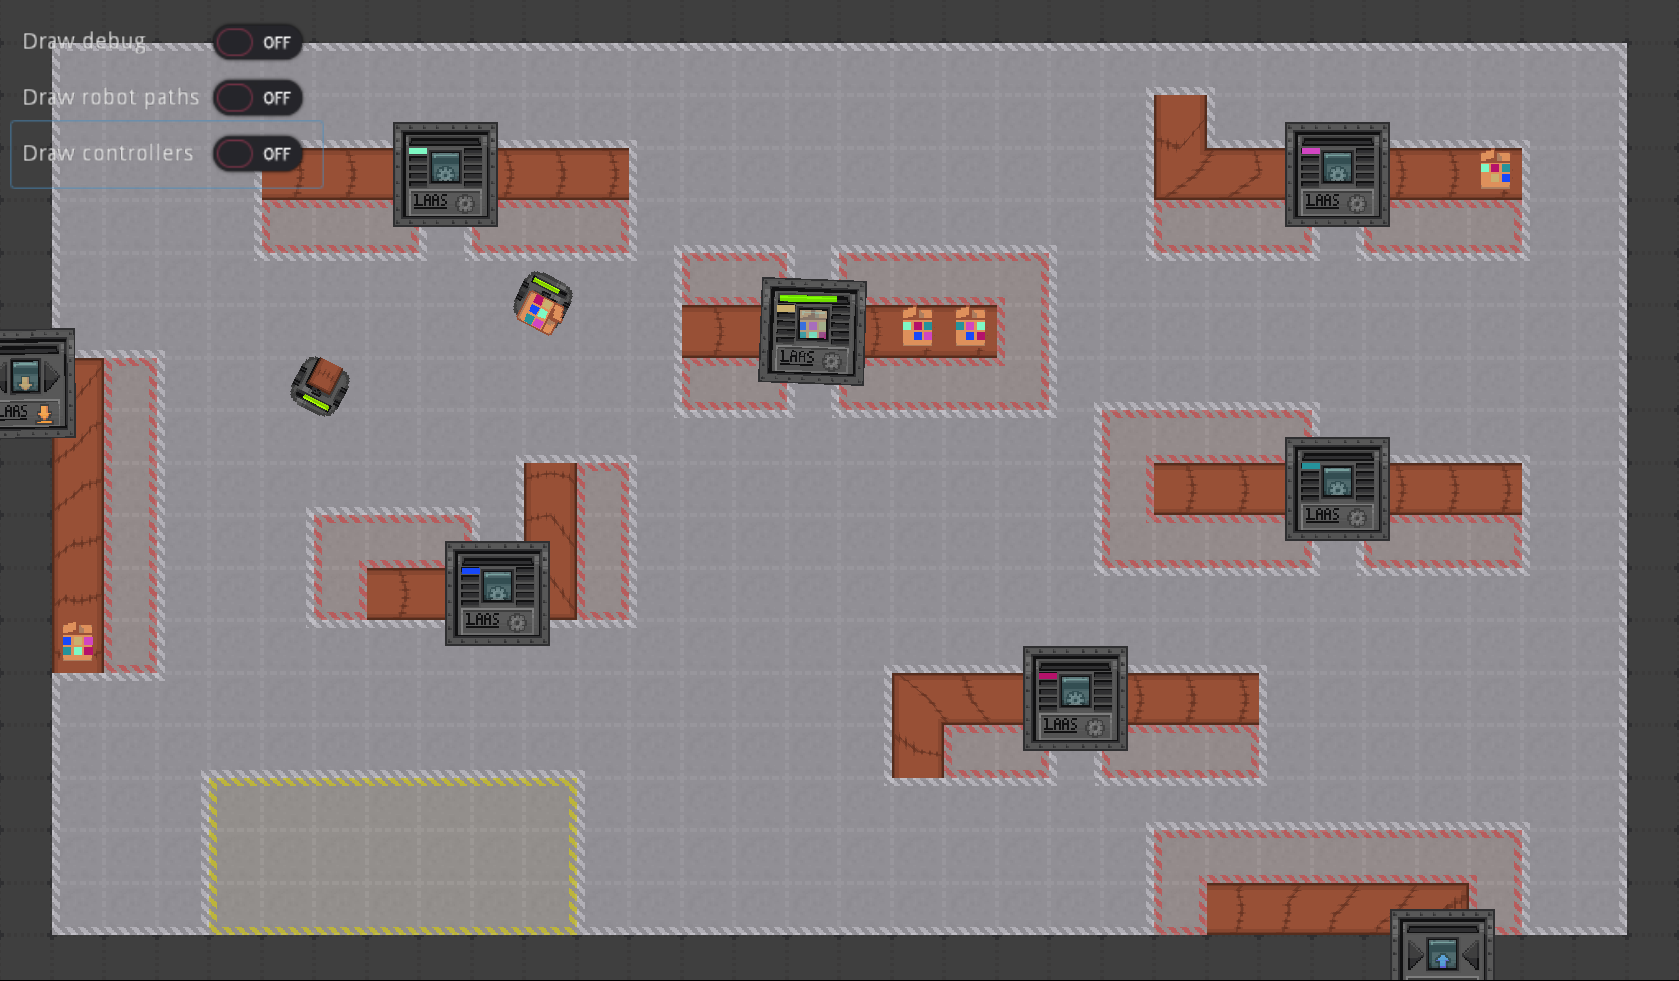
\includegraphics[width=\linewidth]{images/gobot-rae.png}
        \end{column}
    \end{columns}
    
    ~~


    \centering
    \emph{Environment}

~~


    \begin{columns}
        \begin{column}{0.3\textwidth}
            \centering
            Package

            
\includegraphics[width = 0.5\textwidth]{images/godot/package.png}
        \end{column}
        \begin{column}{0.3\textwidth}
            \centering
            Machine

            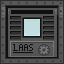
\includegraphics[width = 0.5\textwidth]{images/godot/machine_texture.png}

        \end{column}
        \begin{column}{0.3\textwidth}
            \centering
            Robot

            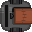
\includegraphics[width = 0.5\textwidth]{images/godot/robot_texture.png}
        \end{column}
    \end{columns}

    % \begin{columns}
    %     \begin{column}{0.2\textwidth}
            
    %     \end{column}
    %     \begin{column}{0.7\textwidth}
    %         Machines
    %         \begin{itemize}
    %             \item Processing : does a predefined list of process for packages
    %             \item Input: generate packages
    %             \item Output: gather fully processed packages
    %         \end{itemize}
    %     \end{column}
    % \end{columns}

    % ~

    % \begin{columns}
    %     \begin{column}{0.2\textwidth}
            
    %     \end{column}
    %     \begin{column}{0.7\textwidth}
    %         Robots : manipulate packages
    %         \begin{itemize}
    %             \item commands: move, pick, place,\dots
    %             \item recharge at recharge areas
    %         \end{itemize}
    %     \end{column}
    % \end{columns}
\end{frame}

% \begin{frame}{Other logistic simulators}
%     \begin{columns}[t]
%         \begin{column}{0.5\textwidth}
%             \small
%             Robocup Logistic League Simulation \cite{niemuellerPlanningCompetitionLogistics2016}

%             \includegraphics[width = \linewidth]{images/robocup.png}
            
%         \end{column}
%         \begin{column}{0.5\textwidth}
%             \small
%             CraftBots \cite{nemiroDesigningAdaptableBenchmark2021}

%             \includegraphics[width = \linewidth]{images/craftbots.png}
%         \end{column}
%     \end{columns}
    
% \end{frame}

\begin{frame}{Mission of the robotic agent}
Mission : Do all the processes of packages.
For each process of a package:
\begin{itemize}
    \item Select a machine to do the process.
    \item Select a robot to carry it to the machine.
\end{itemize}
% ~

%     Role of the autonomous agent:
%     \begin{itemize}
%         \item Control individual AMR.
%         \item Deal with contingencies and errors,
%         \item Optimize choices in function of time and energy.
%     \end{itemize}
\end{frame}
\subsection{Programming the autonomous agent}

\begin{frame}{Programming the autonomous agent}
    Hierarchical representation of the agent skills.
    \begin{itemize}
        \item Different methods for adapted to various contexts.
        \item Different levels of modelling and abstraction $\rightarrow$ ease deliberation.
    \end{itemize}
   
\end{frame}

\begin{frame}{Procedure based system}
    Refinement-based acting with the Refinement Acting Engine (RAE) \cite{ghallabAutomatedPlanningActing2016}:
    \begin{itemize}
        \item Procedure-based system.
        \item Monitor procedure and command execution
        \item Support parallel execution.
        \item Refinement at runtime for more reactive systems.
        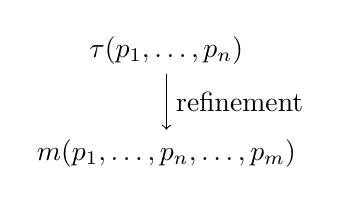
\begin{tikzpicture}
            \node[] (task) {$\tau(p_1,\dots,p_n)$};
            \node[below = 2em of task] (method) {$m(p_1,\dots,p_n, \dots, p_m)$};
            \path[->] (task) edge node[right, midway] {refinement} (method);
        \end{tikzpicture}
    \end{itemize}
\end{frame}

\begin{frame}{Hierarchical operational models to represent the capabilities of an agent}

\begin{columns}[T]
    \begin{column}{0.55\textwidth}
        Agent behavior = collection of skills (procedures)
        
        ~
        \pause
        Hierarchical operational models : Acting domain \textbf{$A_\Delta (A, T, M_t)$}
        \small
        \pause
        \begin{itemize}
        
        
         \item[$A$] : commands (low-level) move, grasp
         \pause
         \item[$T$] : tasks (high-level)
         \pause
         \item[$M_t$] : methods: pre-conditions, body (operational model)
         
     \end{itemize}
    \end{column}
    \pause
    \begin{column}{0.45\textwidth}
        \begin{figure}
            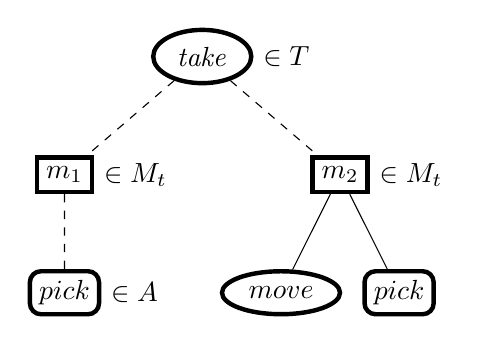
\begin{tikzpicture}
                \node[draw, ellipse, ultra thick] (t) {\textit{take}} [sibling distance = 3.5cm]
                  child {node[draw, ultra thick] (m1) {$m_1$} edge from parent [dashed]
                  child {node[draw,rounded corners, ultra thick, solid] (a1) {$pick$} edge from parent
                  }} 
                  child {node[draw, ultra thick] (m2) {$m_2$} edge from parent [dashed] [sibling distance = 1.5cm]
                  child {node[draw, ellipse, ultra thick, solid] (a2) {$move$} edge from parent [solid]}
                  child {node[draw, rounded corners, solid, ultra thick] {$pick$} edge from parent [solid]}};
                \node[right = 0em of t] {$\in T$};
                \node[right = 0em of m1] {$\in M_t$};
                \node[right = 0em of m2] {$\in M_t$};
                \node[right = 0em of a1] {$\in A$};

            \end{tikzpicture}
            \caption{Example of hierarchy for the \textit{task} \textit{open door}}

            
        \end{figure}
    \end{column}
\end{columns}
    
\end{frame}

\begin{frame}{RAE algorithms}
    \begin{columns}[T]
  
        \begin{column}{0.65\textwidth}
            
            Algorithms:
            \small
            \begin{itemize}
                \setlength{\leftmargini}{-1pt}
                \onslide<2->
                \item \textbf{Main:} 
                \begin{itemize}
                    \item Receive $\tau$ (task or event);
                    
                    add it to the \textbf{agenda} (ongoing tasks)
                    \onslide<3->
                    \item Refine $\tau$: \textbf{Select} an applicable method $m$ for $\tau$
                    \onslide<4->
                    \item \textbf{Progress} $m$
                \end{itemize}
                \onslide<5->
                \item \textbf{Progress:}
                    \begin{itemize}
                        \onslide<6->
                        \item Monitor execution of $m$.
                        \onslide<7->
                        \item Refine subtasks in $m$.    
                        \onslide<8->
                        \item Monitor execution of subtasks.
                        \onslide<9->
                        \item \textbf{Retry} $\tau$ in case of \emph{failure}:
                    
                    Call \textbf{Select} to get a new method;
                    
                    \textbf{Progress} the new method.
                    \end{itemize}
            \end{itemize}
        \end{column}
        \begin{column}{0.35\textwidth}
            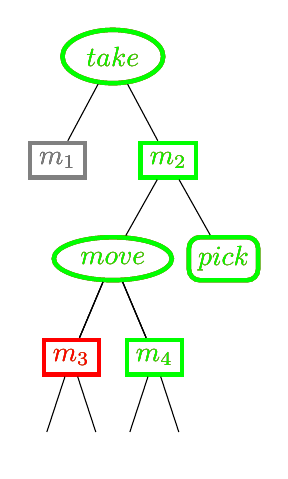
\begin{tikzpicture}
                \onslide<2>
                \node[draw,ellipse, ultra thick] (t) {$take$};
                \onslide<3-9>
                \node[draw,ellipse, ultra thick, color = orange] (t) {$take$};
                \onslide<10>
                \node[draw,ellipse, ultra thick, color = green] (t) {$take$};
                \onslide<3>
                \node[draw, ultra thick, below= 2em of t, xshift = -2em] (m1) {$m_1$};
                \node[draw, ultra thick, below= 2em of t, xshift = 2em] (m2) {$m_2$};
                \onslide<4->
                \node[draw, ultra thick, below= 2em of t, xshift = -2em, color = gray] (m1) {$m_1$};
                \node[draw, ultra thick, below= 2em of t, xshift = 2em, color = orange] (m2) {$m_2$};
                \onslide<10>
                \node[draw, ultra thick, below= 2em of t, xshift = 2em, color = green] (m2) {$m_2$};
                \onslide<3->
                \path[-] (t) edge (m1) (t) edge (m2);
                \onslide<5>
                \node[draw,rounded corners, ultra thick, solid, below = 2em of m2, xshift = 2em] (a1) {$pick$};
                \onslide<6>
                \node[draw,rounded corners, ultra thick, solid, below = 2em of m2, xshift = 2em, color = orange] (a1) {$pick$};
                \onslide<7->
                \node[draw,rounded corners, ultra thick, solid, below = 2em of m2, xshift = 2em, color = green] (a1) {$pick$};
                \onslide<5-7>
                \node[draw,ellipse, ultra thick, solid, below = 2em of m2, xshift = -2em] (t2) {$move$};
                \onslide<8->
                \node[draw,ellipse, ultra thick, solid, below = 2em of m2, xshift = -2em, color = orange] (t2) {$move$};
                \onslide<10>
                \node[draw,ellipse, ultra thick, solid, below = 2em of m2, xshift = -2em, color = green] (t2) {$move$};
  
  
                \onslide<5->
                \path[-] (m2) edge (a1) (m2) edge(t2);
  
  
                \onslide<7>
                \node[draw, ultra thick, below = 2em of t2, xshift = -1.5em] (m3) {$m_3$};
                \node[draw, ultra thick, below = 2em of t2, xshift = 1.5em] (m4) {$m_4$};
                \path[-] (t2) edge  (m3) (t2) edge (m4);
                
                \onslide<8>
                \node[draw, ultra thick, below = 2em of t2, xshift = -1.5em, color = orange] (m3) {$m_3$};
                \node[draw, ultra thick, below = 2em of t2, xshift = 1.5em, color = gray] (m4) {$m_4$};
                \path[-] (t2) edge  (m3) (t2) edge (m4);
  
                \onslide<9->
                \node[draw, ultra thick, below = 2em of t2, xshift = -1.5em, color = red] (m3) {$m_3$};
                \node[draw, ultra thick, below = 2em of t2, xshift = 1.5em, color = orange] (m4) {$m_4$};
                \path[-] (t2) edge  (m3) (t2) edge (m4);
                \onslide<10>
                \node[draw, ultra thick, below = 2em of t2, xshift = 1.5em, color = green] (m4) {$m_4$};
                
                \onslide<8->
                \node[below = 2em of m3, xshift = -1em] (e3) {};
                \node[below = 2em of m3, xshift = 1em] (e4) {};
                \path[-] (m3) edge  (e3) (m3) edge (e4);
  
                \onslide<8->
                \node[below = 2em of m4, xshift = -1em] (e5) {};
                \node[below = 2em of m4, xshift = 1em] (e6) {};
                \path[-] (m4) edge  (e5) (m4) edge (e6);
      
            \end{tikzpicture}
        \end{column}
    \end{columns}    
\end{frame}



\begin{frame}[fragile]{Simple scenario: one package}
    \centering
    \begin{columns}
        \begin{column}{0.5\textwidth}
            \centering
            
\includegraphics[width = 0.3\textwidth]{images/godot/package.png}
            
            \LARGE \emph{$\times 1$}
        \end{column}
        \begin{column}{0.5\textwidth}
            \centering
            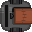
\includegraphics[width = 0.3\textwidth]{images/godot/robot_texture.png}
            
            \LARGE \emph{$\times 1$}
        \end{column}
    \end{columns}
    \pause
    \begin{itemize}
        \item task: process(?p)
        \item methods:
    \end{itemize}
    \footnotesize
    \begin{columns}[t]
        \begin{column}{0.32\textwidth}
            m1(?p, ?r, ?m)
            \begin{align*}
                pre: &\ proc(?p) \neq \emptyset \\
                 &battery(?r) > 40\% \\
                 &proc(?p)[1] \in proc(?m) \\
                 body:&take(?p,?r) \\
                     &carry(?p,?r,?m) \\
                     &process(?p)
            \end{align*}
        \end{column}
        \begin{column}{0.32\textwidth}
            m2(?p, ?r, ?m)
            \begin{align*}
                pre: &\ proc(?p)  = \emptyset \\
                 &battery(?r) > 40\% \\
                 &kind(?m) = \text{output} \\
                 body:&take(?p,?r) \\
                     &carry(?p,?r,?m) \\
            \end{align*}
        \end{column}
        \begin{column}{0.32\textwidth}
            m3(?p, ?r) 
            \begin{align*}  
                pre: &battery(?r) \leq 40\% \\
                 body:&recharge(?r) \\
                     &process(?p)
            \end{align*}
        \end{column}
    \end{columns}
    % \begin{align*}
    %     \text{task:} & \text{process(?p)}\\
    %     \text{methods:}& \\
    %     m1(?p, ?r, ?m) \\
    %     \text{pre:} & !empty(processes(?p)) \\
    %      &battery(?r) \leq 40\% \\
    %      &first(processes(?p)) \in processes(?m) \\
    %      body:&take(?p,?r) \\
    %          &carry(?p,?r,?m) \\
    %          &process(?p)
    % \end{align*}
    
\end{frame}

\begin{frame}{Running example with one package}
    \LARGE
    \centering
    \href{https://youtu.be/a4_tITUTQuQ}{Video example}
\end{frame}

\subsection{Multi-agent scenario}

\begin{frame}{Several packages?}
    \begin{columns}
        \begin{column}{0.5\textwidth}
            \centering
            
\includegraphics[width = 0.5\textwidth]{images/godot/package.png}
            
            \Large $\times n$
        \end{column}
        \begin{column}{0.5\textwidth}
            \centering
            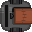
\includegraphics[width = 0.5\textwidth]{images/godot/robot_texture.png}
            
            \LARGE $\times m$
        \end{column}
    \end{columns}
    
    ~

    New decisions for the robotic system:
    \begin{itemize}
        \item Schedule package passage on machines
        \item Allocate package displacement tasks to robots
        %\item Monitor the robots' batteries 
    \end{itemize}

    \centering
\end{frame}

\begin{frame}{Multi-agent refinement-based deliberation}
    \begin{columns}[t]
        \begin{column}{0.45\textwidth}
            RAE shortcomings:
            \begin{itemize}
                \item Progression of tasks relies on Round Robin
                \item Methods limited to a sequence of actions
                %\item Difficulties to integrate sound planning from operational models due to implementation in Python.
            \end{itemize}
        \end{column}
        \begin{column}{0.1\textwidth}
            $\rightarrow$

        \end{column}
        \begin{column}{0.45\textwidth}
            Adapt RAE for multi-agents to
            \begin{itemize}
                \item Deal with concurrency
                \item Improve the interleaving of parallel tasks
                \item Reason on shared resources to optimize the overall process
            \end{itemize}
        \end{column}
    \end{columns}
\end{frame}
\section{Acting for multi-agents}
\subsection{Deliberative acting}
\begin{frame}{Definition of a robotic agent}

    \begin{columns}[T]
        \begin{column}{0.3\textwidth}
            An entity

            ~

            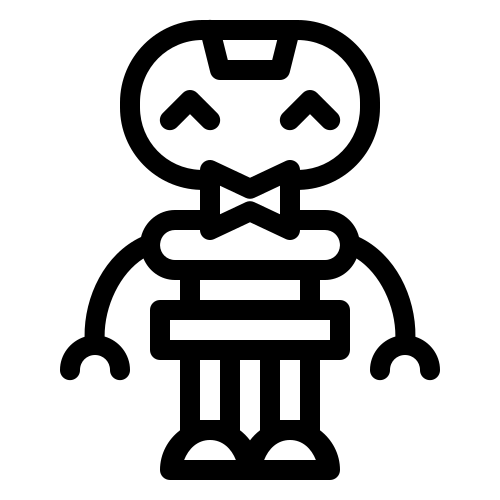
\includegraphics[width = 0.7\textwidth]{images/icons8-robot-gustav-500.png}
        \end{column}
        \begin{column}{0.7\textwidth}
            \center Capable of :
            \pause
            \begin{enumerate}
                \item Perceiving its environment
                \pause
                \item Modifying its environment (actions)
                \pause
                \item \textbf{Deliberating:} Reasoning about its \textbf{skills} in order to fulfill a goal
            \end{enumerate}
        \end{column}
    \end{columns}

 
\end{frame}

\begin{frame}{Representing the skills of an agent}

\begin{columns}[T]
    \begin{column}{0.55\textwidth}

        \begin{itemize}
            \item Elementary capabilities : move, grasp, look, \dots
            \pause
            \item Skills : executable programs (operational models): set the table, \dots
            \pause
            \item Robot behavior = composition of skills
        \end{itemize}
        
        ~
        \pause
        Acting domain \textbf{$A_\Delta (A, T, M_t)$}: Hierarchical operational models
        \small
        \pause
        \begin{itemize}
        
        
         \item[$A$] : primitive tasks
         \pause
         \item[$T$] : abstract tasks
         \pause
         \item[$M_t$] : methods: pre-conditions, body (operational model)
         
     \end{itemize}
    \end{column}
    \pause
    \begin{column}{0.45\textwidth}
        \begin{figure}
            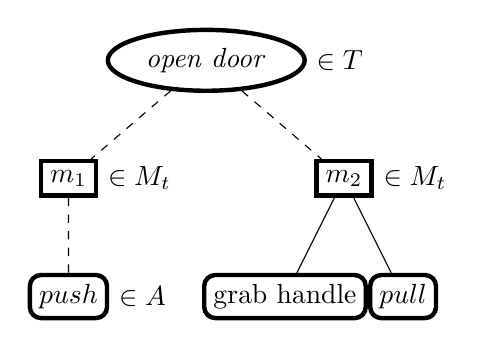
\begin{tikzpicture}
                \node[draw,ellipse, ultra thick] (t) {\textit{open door}} [sibling distance = 3.5cm]
                  child {node[draw, ultra thick] (m1) {$m_1$} edge from parent [dashed]
                  child {node[draw,rounded corners, ultra thick, solid] (a1) {$push$} edge from parent
                  }} 
                  child {node[draw, ultra thick] (m2) {$m_2$} edge from parent [dashed] [sibling distance = 1.5cm]
                  child {node[draw, rounded corners, solid, ultra thick] (a2) {grab handle} edge from parent [solid]}
                  child {node[draw, rounded corners, solid, ultra thick] {$pull$} edge from parent [solid]}};
                \node[right = 0em of t] {$\in T$};
                \node[right = 0em of m1] {$\in M_t$};
                \node[right = 0em of m2] {$\in M_t$};
                \node[right = 0em of a1] {$\in A$};

            \end{tikzpicture}
            \caption{Example of hierarchy for the \textit{task} \textit{open door}}

            
        \end{figure}
    \end{column}
\end{columns}
    
\end{frame}

\begin{frame}{Refinement Acting Engine (RAE)\footnote{Automated Planning and Acting \cite{ghallabAutomatedPlanningActing2016}}: deliberation algorithms using hierarchical operational models}
    RAE features:
    \begin{itemize}
        \item Hierarchical representation of the agent skills.
        \item Refinement at runtime:
        \centering
        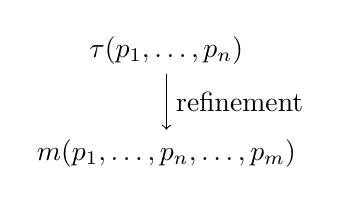
\begin{tikzpicture}
            \node[] (task) {$\tau(p_1,\dots,p_n)$};
            \node[below = 2em of task] (method) {$m(p_1,\dots,p_n, \dots, p_m)$};
            \path[->] (task) edge node[right, midway] {refinement} (method);
        \end{tikzpicture}
        \item Monitoring command and task execution.
        \item Perform multiple tasks in parallel
        \pause
        \item Automated deliberation: Refinement of task into method and choice of parameters
    \end{itemize}    
\end{frame}
    

\begin{frame}{Refinement Acting Engine algorithms}
    \begin{columns}[T]
  
        \begin{column}{0.65\textwidth}
            
            Algorithms:
            \small
            \begin{itemize}
                \setlength{\leftmargini}{-1pt}
                \onslide<2->
                \item \textbf{Main:} 
                \begin{itemize}
                    \item Receive $\tau$ (task or event);
                    
                    add it to the \textbf{agenda} (ongoing tasks)
                    \onslide<3->
                    \item Refine $\tau$: \textbf{Select} an applicable method $m$ for $\tau$
                    \onslide<4->
                    \item \textbf{Progress} $m$
                \end{itemize}
                \onslide<5->
                \item \textbf{Progress:}
                    \begin{itemize}
                        \onslide<6->
                        \item Monitor execution of $m$.
                        \onslide<7->
                        \item Refine subtasks in $m$.    
                        \onslide<8->
                        \item Monitor execution of subtasks.
                        \onslide<9->
                        \item \textbf{Retry} $\tau$ in case of \emph{failure}:
                    
                    Call \textbf{Select} to get a new method;
                    
                    \textbf{Progress} the new method.
                    \end{itemize}
            \end{itemize}
        \end{column}
        \begin{column}{0.35\textwidth}
            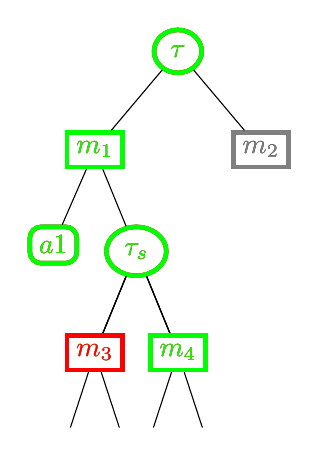
\begin{tikzpicture}
                \onslide<2>
                \node[draw,ellipse, ultra thick] (t) {$\tau$};
                \onslide<3-9>
                \node[draw,ellipse, ultra thick, color = orange] (t) {$\tau$};
                \onslide<10>
                \node[draw,ellipse, ultra thick, color = green] (t) {$\tau$};
                \onslide<3>
                \node[draw, ultra thick, below= 2em of t, xshift = -3em] (m1) {$m_1$};
                \node[draw, ultra thick, below= 2em of t, xshift = 3em] (m2) {$m_2$};
                \onslide<4->
                \node[draw, ultra thick, below= 2em of t, xshift = -3em, color = orange] (m1) {$m_1$};
                \node[draw, ultra thick, below= 2em of t, xshift = 3em, color = gray] (m2) {$m_2$};
                \onslide<10>
                \node[draw, ultra thick, below= 2em of t, xshift = -3em, color = green] (m1) {$m_1$};
                \onslide<3->
                \path[-] (t) edge (m1) (t) edge (m2);
                \onslide<5>
                \node[draw,rounded corners, ultra thick, solid, below = 2em of m1, xshift = -1.5em] (a1) {$a1$};
                \onslide<6>
                \node[draw,rounded corners, ultra thick, solid, below = 2em of m1, xshift = -1.5em, color = orange] (a1) {$a1$};
                \onslide<7->
                \node[draw,rounded corners, ultra thick, solid, below = 2em of m1, xshift = -1.5em, color = green] (a1) {$a1$};
                \onslide<5-7>
                \node[draw,ellipse, ultra thick, solid, below = 2em of m1, xshift = 1.5em] (t2) {$\tau_s$};
                \onslide<8->
                \node[draw,ellipse, ultra thick, solid, below = 2em of m1, xshift = 1.5em, color = orange] (t2) {$\tau_s$};
                \onslide<10>
                \node[draw,ellipse, ultra thick, solid, below = 2em of m1, xshift = 1.5em, color = green] (t2) {$\tau_s$};
  
  
                \onslide<5->
                \path[-] (m1) edge (a1) (m1) edge(t2);
  
  
                \onslide<7>
                \node[draw, ultra thick, below = 2em of t2, xshift = -1.5em] (m3) {$m_3$};
                \node[draw, ultra thick, below = 2em of t2, xshift = 1.5em] (m4) {$m_4$};
                \path[-] (t2) edge  (m3) (t2) edge (m4);
                
                \onslide<8>
                \node[draw, ultra thick, below = 2em of t2, xshift = -1.5em, color = orange] (m3) {$m_3$};
                \node[draw, ultra thick, below = 2em of t2, xshift = 1.5em, color = gray] (m4) {$m_4$};
                \path[-] (t2) edge  (m3) (t2) edge (m4);
  
                \onslide<9->
                \node[draw, ultra thick, below = 2em of t2, xshift = -1.5em, color = red] (m3) {$m_3$};
                \node[draw, ultra thick, below = 2em of t2, xshift = 1.5em, color = orange] (m4) {$m_4$};
                \path[-] (t2) edge  (m3) (t2) edge (m4);
                \onslide<10>
                \node[draw, ultra thick, below = 2em of t2, xshift = 1.5em, color = green] (m4) {$m_4$};
                
                \onslide<8->
                \node[below = 2em of m3, xshift = -1em] (e3) {};
                \node[below = 2em of m3, xshift = 1em] (e4) {};
                \path[-] (m3) edge  (e3) (m3) edge (e4);
  
                \onslide<8->
                \node[below = 2em of m4, xshift = -1em] (e5) {};
                \node[below = 2em of m4, xshift = 1em] (e6) {};
                \path[-] (m4) edge  (e5) (m4) edge (e6);
      
            \end{tikzpicture}
        \end{column}
    \end{columns}    
\end{frame}
\subsection{OMPAS: Extending RAE for fleet management}

\begin{frame}{Multi-agent: extending RAE definition for concurrency}
    \begin{columns}
        \begin{column}{0.5\textwidth}
            RAE shortcomings:
            \begin{itemize}
                \item Progression of tasks relies on Round Robin
                \item Methods limited to a sequence of actions
                \item Difficulties to integrate sound planning from operational models due to implementation in Python.
            \end{itemize}
        \end{column}
        \begin{column}{0.5\textwidth}
            RAE extension:
            \begin{itemize}
                \item Progression handled by a scheduler
                \item Complex method bodies:
                \begin{itemize}
                    \item Concurrency inside methods
                    \item General programming constructs
                    \item error and interruption handling
                \end{itemize}
                \item Reasoning on shared resources for the interleaving of tasks.
            \end{itemize}
        \end{column}
    \end{columns}
\end{frame}

\begin{frame}{Adaptation of the main algorithm}
    \begin{itemize}
        \item Each task is evaluated in its own thread.
        \item Shared objects among all threads: state, resources
    \end{itemize}
  
    \tikzstyle{thread} = [draw, rounded corners, rectangle, fill=black!50]
    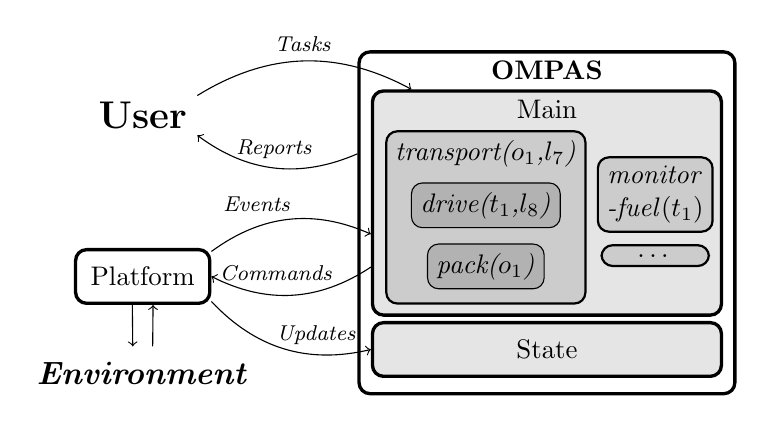
\begin{tikzpicture}[scale=0.97, every node/.style={scale=0.97}]
  
        %RAE
        \node[draw = black, very thick,
            minimum width = 14em,
            minimum height = 5em,
            rounded corners,
            text = black,
            text centered, text depth = 4 cm,
            align = center,
            ] (R) at (0,0) {\textbf{OMPAS}};
        %Operational Models
        % \node[draw = black, ellipse, very thick,
        %     minimum width = 7em,
        %     minimum height = 2em,
        %     above = 1em of R,
        %     text = black,
        %     text centered, align=center
        % ] (OM) {\textit{Operational Models} %($A_\Delta$)
        % };
  
  
        %state
        \node[draw = black, very thick,
        text centered,
        minimum width = 13em,
        minimum height = 2em,
        rounded corners,
        text = black,
        fill=black!10,
        align = center] (S) at ($(R.south) + (0,0.6)$) {State};
  
        %main
        \node[draw = black, very thick,
        minimum height = 8em,
        minimum width = 13em,
        rounded corners,
        text = black,
        text centered, text depth = 7em,
        fill=black!10,
        align=center] (main) at ($(R.north) + (0,-2)$) {Main};
  
        %t1
        \node[draw = black, thick,
        minimum height = 6em,
        minimum width = 7em,
        rounded corners,
        text = black,
        text centered, text depth = 5em,
        fill=black!20,
        align=center](t1) at ($(main.south) + (-0.8, 1.3)$) {\emph{transport($o_1$,$l_7$)}};
  
  
        %first task
        \node[draw, rounded corners, rectangle, fill=black!30] (st11) at ($(t1.south) + (0,1.3)$) {\emph{drive($t_1$,$l_8$)}};
        \node[draw, rounded corners, rectangle, fill=black!30] (st12) at ($(st11.south) + (0,-.5)$){\emph{pack($o_1$)}};
        
        \node[draw, thick, rounded corners, rectangle,minimum width = 4em, fill=black!20, align= center] (t3) at ($(t1.east) + (0.9, 0.3)$){\textit{monitor}\\
        \textit{-fuel}($t_1$)};
        \node[draw, thick, rounded corners, rectangle,minimum width = 4em, fill=black!20, align= center] (t3) at ($(t1.east) + (0.9, -0.5)$){\dots};
  
  
  
        %platform
        \node[draw = black, very thick,
        text centered,
        minimum width = 5em,
        minimum height = 2em,
        %below = 2em of R,
        rounded corners,
        text = black,
        align = center,] (Pl) at ($(R.west) +(-8em, -2em)$) {Platform};
  
        \node[text centered,
        minimum width = 5em,
        minimum height = 2em,
        below = 1.5em of Pl,
        rounded corners,
        text = black,
        align = center,] (E) {\textbf{\large\textit{Environment}}};
  
        \node[very thick,
            text centered,
            rounded corners,
            text = black] (U) at ($(R.west) +(-8em, +4em)$) {\Large \textbf{User}};
        
        % \node[draw = black, very thick,
        %     text centered,
        %     right = 7em of R,
        %     minimum width = 5em,
        %     minimum height = 4em,
        %     rounded corners,
        %     text = black] (Pl) {Platform};
        
  
        \path[->]
  
            %Link between operational models library
            %(OM) edge (R)
  
            (U.20) edge[bend left] node [midway, above, align=center] {\footnotesize \emph{Tasks}} (main.+140)
            (R.+160) edge [bend left] node [midway, above] {\footnotesize \emph{Reports}} (U.-20)
        
            %Link between RAE and the platform
            (main.-160) edge[bend left] node [pos = 0.6, above = 0.2em] {\footnotesize \emph{Commands}} (Pl.east)
            
            %between platform and state
            (Pl.-20) edge [bend right] node [pos = 0.7, right, above, align = center] {\footnotesize \emph{Updates}} (S.west)
            
            %between platform and main
            (Pl.20) edge [bend left] node [pos = 0.3, right, above= 0.2em, align = center] {\footnotesize \emph{Events}} (main.-170)
  
            (Pl.-110) edge (E.110)
            (E.70) edge (Pl.-70)
            ;
        
        \end{tikzpicture}

\end{frame}

\subsection{An acting language based on Scheme}
\begin{frame}{SOMPAS: A Lisp variant with acting primitives}
    
    \begin{columns}
        \begin{column}{0.5\textwidth}
            Why Scheme?
            \begin{itemize}
                \item Few primitives
                \item Functional
                \item Generic programming constructs
                \item Identified and simple semantic $\rightarrow$ suitable to automated analysis for planning
            \end{itemize}
        \end{column}
        \begin{column}{0.5\textwidth}
            Features :
            \begin{itemize}
                \item Concurrency and interruption
                \item Acting primitives
                \item Resource acquisition mechanism for synchronization and exclusion.
            \end{itemize}

        \end{column}
    \end{columns}
\end{frame}

\begin{frame}[fragile]{Concurrency and interruption}
    handle: new LValue
    Functions:
    \begin{itemize}
        \item \textit{(async e)}: creates a new thread to evaluate e, returns a handle
        \item \textit{(await h)}: awaits the result of the concurrent evaluation.
        \item \textit{(interrupt h)}: interrupts the concurrent evaluation.
    \end{itemize}
    
\begin{columns}
    \begin{column}{0.4\textwidth}
        \lstset{basicstyle=\footnotesize, columns=fullflexible}
\begin{lstlisting}[language=lisp]
(begin
 (define h
  (async 
    (begin
     (uninterruptible (begin
       (exec pick ?r ?o)
       (exec move ?r ?l)
       (exec drop ?r ?o)))
     (exec inspect ?r ?o))))
 (race 
   (await h)
   (begin
    (sleep 10)
    (interrupt h))))
\end{lstlisting}

    \end{column}
    \begin{column}{0.6\textwidth}
        \newcommand{\Cross}{$\mathbin{\tikz [x=1.4em,y=1.4em,line width=.2em, red] \draw (0,0) -- (1,1) (0,1) -- (1,0);}$}
    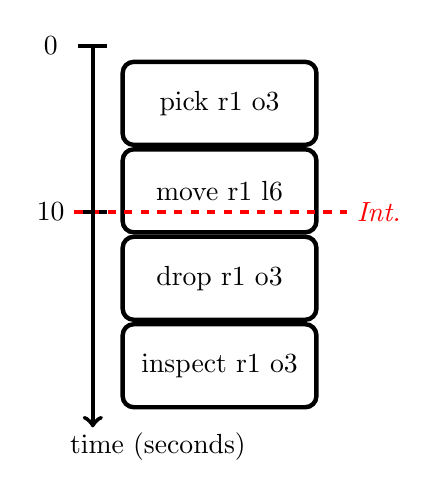
\begin{tikzpicture}
        \node[draw,
        rounded corners,
        ultra thick,
        minimum height = 3em,
            minimum width = 7em,] (pick) at (0,0) {pick r1 o3};
    
        \node[draw, rounded corners,
        ultra thick,
            minimum height = 3em,
            minimum width = 7em,
        ] (move) at ($1.5*(pick.south)-0.5*(pick.north)$) {move r1 l6};
        %\action{move, move r1 l6, 10em, pick}
    
        \node[draw, rounded corners,
        ultra thick,
            minimum height = 3em,
            minimum width = 7em,
        ] (drop) at ($1.5*(move.south) - 0.5*(move.north)$) {drop r1 o3};
        \node[draw, rounded corners,
        ultra thick,
            minimum height = 3em,
            minimum width = 7em,
        ] (inspect) at ($1.5*(drop.south) - 0.5*(drop.north)$) {inspect r1 o3};
        \node at (inspect) {\Cross};
    
            \node[] (origin) at ($(pick.north west) + (-1em,+0.5em)$) {~~};
        
            \node[] (zero) at ($(origin.west) + (-1em,0)$) {0};
            \draw[-, ultra thick] (origin.west) -- (origin.east);
            \node[] (ten) at ($(zero) + (0,-6em)$) {10};
            \draw[-, ultra thick] ($(origin.west) + (0,-6em)$) -- ($(origin.east) + (0,-6em)$);
    
    
            \node[] (interruption) at ($(ten.east) +(11em,0em)$){\color{red} \textit{Int.}};%{\color{red} \textit{interruption}};
            \draw[-, ultra thick, dashed, color= red] ($(ten.east)$) -- ( interruption);
            \node[] (end) at ($1.5*(inspect.south west) - 0.5*(inspect.south west) + (-1em,-1em)$) {};
            \node[] (time) at ($1.5*(end.south east) - 0.5*(end.south east) + (2em,0)$)  {time (seconds)};
    
    
        \path[->] (origin.center) edge[ultra thick] (end);
    \end{tikzpicture}
    \end{column}
\end{columns}    
\end{frame}

\begin{frame}{Acting primitives}
    \begin{itemize}
    \pause
        \item \textit{(exec a $p_1...p_n$)} executes and monitors a task or command.
    \pause
        \begin{itemize}
            \item command : resorts to the platform
            \item task: selects a method and execute its operational model.
        \end{itemize}
    \pause
        \item \textit{(read-state sf $p_1...p_n$)} returns the value of a state-variable
        \item \textit{(arbitrary set $\lambda$)} returns an arbitrary element from a $set$. $\lambda$ can be used to select among the $set$.
    \end{itemize}
\end{frame}

\begin{frame}[t]{Resources}
    \begin{columns}
        \begin{column}{0.5\textwidth}
            Definition of a resource:
            \begin{itemize}
                \item Object with initial capacity $C_{init}$
                \item Acquire $r$ at $t$ with amount $c$: $c \leq C_t$ 
            \end{itemize}
            Kinds of resources : 
            \begin{itemize}
                \item \emph{unary}: $C_{init} = 1$, $c = 1$;
                \item \emph{divisible}: $C_{init} \in  \mathbb{R}_+^*$, $c \in ]0, C_t]$
            \end{itemize}
        \end{column}
        \begin{column}{0.5\textwidth}
            Functions
            \begin{itemize}
                \item \textit{(new-resource r C)}: declare a new resource with a label and a capacity.
                \item \emph{(acquire r c)} request the acquisition of $r$ with amount $c$. Returns a resource-handle
                \item \emph{(release h)} release the resource of the resource-handle
            \end{itemize}
        \end{column}
    \end{columns}
\end{frame}

\begin{frame}{More advanced features and programming constructs}
    More complex behavior definition
    \begin{itemize}
        \item \textit{(wait-for dyn)} waits until the expression \textit{dyn} becomes true 
        \item \textit{(run-monitoring e dyn)} evaluates \textit{e} while \textit{dyn} is true, interrupts \textit{e} otherwise.
        \item ...
    \end{itemize}
\end{frame}

\begin{frame}[t,fragile]{Defining an acting domain with SOMPAS}
    \setlength{\leftmargini}{0pt}
    \begin{columns}
        \begin{column}{0.5\textwidth}
            \begin{itemize}
                \footnotesize
                \item Task (label, typed parameters):
                \tiny
                \begin{lstlisting}
(def-task t_process_package
    (:params (?p package)))
                \end{lstlisting}
                \footnotesize
                \pause
                \item Method (label, typed parameters, pre-conditions, body):
                \tiny
                \begin{lstlisting}
(def-method m_process_to_do_r
  (:task t_process_package)
  (:params (?p package))
  (:pre-conditions
    (!= (package.processes_list ?p)
        nil)))
  (:body
    (do
     (define ?m ...)
     (t_process_on_machine ?p ?m)
     (t_process_package ?p)))   
                \end{lstlisting}
            \end{itemize}
        \end{column}
    \pause
        \begin{column}{0.5\textwidth}
            \begin{itemize}
    \pause
            \footnotesize
            \item State-function (label, typed parameters \& result):
            \tiny
            \begin{lstlisting}
(def-state-function at
    (:params (?r robot))
    (:result location))
            \end{lstlisting}
    \pause
            \footnotesize
            \item Command (label, typed parameters):
            \tiny
            \begin{lstlisting}
(def-command pick (:params (?r robot)))
                \end{lstlisting}
            \end{itemize}

    \pause
            ~
        \normalsize
        Others:
        
        \textit{lambda, type, constant}
        \end{column}

    \end{columns}
\end{frame}
\section{Results for a logistic simulator}


\begin{frame}[fragile]{OMPAS models for GobotSim}
    \begin{columns}
        \begin{column}{0.5\textwidth}
            \begin{itemize}
                \item High-level goal: process all packages in the environment
                \item Body of the unique method of the high-level task.
                \setlength{\leftmargini}{0pt}
    
                \tiny
            \begin{lstlisting}
    (do
    (mapf new-resource (instance robot))
    (mapf new-resource (instance machine))
    (define h1 (async (t_process_packages)))
    (define h2 (async (t_check_rob_bat)))
    (await h1))
            \end{lstlisting}    
            \end{itemize}
    
    
            
        \end{column}
        \begin{column}{0.5\textwidth}
    \end{column}
    \end{columns}
    
    \end{frame}

\begin{frame}{Validation on Job shop problems}
\centering
%Outline the features of the new system and the language
\begin{columns}
    \begin{column}{0.5\textwidth}
        Restriction of the simulation:
        \begin{itemize}
            \item All packages are created at the beginning
            \item Each machine can do a unique process
        \end{itemize}
    \end{column}
    \begin{column}{0.5\textwidth}
        Different strategies:
        \begin{itemize}
            \item Greedy
            \item Advanced
            \item ALRPTF
        \end{itemize}
    \end{column}
\end{columns}
\end{frame}

\newcommand{\calcrowmean}{
    \def \rowmean{0}
    \pgfmathparse{\pgfkeysvalueof{/pgfplots/table/summary statistics/end index}-\pgfkeysvalueof{/pgfplots/table/summary statistics/start index}+1}
    \edef\numberofcols{\pgfmathresult}
            % ... loop over all columns, summing up the elements
    \pgfplotsforeachungrouped \col in {1,2,3,4,5,6,7,8,9,10}% in {\pgfkeysvalueof{/pgfplots/table/summary statistics/start index},...,\pgfkeysvalueof{/pgfplots/table/summary statistics/end index}}
    {
        
        \typeout{col = \col}
        
        \pgfmathparse{\rowmean+\thisrowno{\col}/\numberofcols}
        \edef \rowmean{\pgfmathresult}
    }
}
\newcommand{\calcstddev}{
    \def\rowstddev{0}
    \calcrowmean
    \pgfplotsforeachungrouped \col in {1,2,3,4,5,6,7,8,9,10}
    % {\pgfkeysvalueof{/pgfplots/table/summary statistics/start index},...,\pgfkeysvalueof{/pgfplots/table/summary statistics/end index}}
    {
        \pgfmathparse{\rowstddev+(\thisrowno{\col}-\rowmean)^2/(\numberofcols-1)}
        \edef\rowstddev{\pgfmathresult}
    }
    \pgfmathparse{sqrt(\rowstddev)}
}
\newcommand{\calcstderror}{
    \calcrowmean
    \calcstddev
    \pgfmathparse{sqrt(\rowstddev)/sqrt(\numberofcols)}
}

\pgfplotstableset{
    summary statistics/start index/.initial=1,
    summary statistics/end index/.initial=10,
    create col/mean/.style={
        /pgfplots/table/create col/assign/.code={% In each row ... 
            \calcrowmean
            \pgfkeyslet{/pgfplots/table/create col/next content}\rowmean
        }
    },
    create col/standard deviation/.style={
        /pgfplots/table/create col/assign/.code={% In each row ... 
            \calcstddev
            \pgfkeyslet{/pgfplots/table/create col/next content}\pgfmathresult
        }
    },
    create col/standard error/.style={
        create col/assign/.code={% In each row ... 
            \calcstderror
            \pgfkeyslet{/pgfplots/table/create col/next content}\pgfmathresult
        }
    }
}

\pgfplotstableset{
    create on use/mean/.style={create col/mean},
    create on use/stddev/.style={create col/standard deviation},
    create on use/stderror/.style={create col/standard error}
}



\begin{frame}{Results comparison}
    \begin{figure}[t]

        \begin{tikzpicture}
          \begin{axis}[
                      /pgf/number format/.cd,
                          use comma,
                      height = 6cm,
                      width = \linewidth,
                      ymajorgrids,
                      ylabel={Time in seconds},
                      xlabel={Problems},
                      ymin = 0,
                      ymax= 220,
                      ybar=0pt,
                      bar width=12pt,
                      enlarge x limits = 0.3,
                      nodes near coords,
                      point meta=explicit symbolic,
                      scatter/position=absolute,
                      every node near coord/.style={
                              at={(\pgfkeysvalueof{/data point/x},1.8)},
                              anchor=south,
                          },
                      bar shift=0pt,
                      xtick={0,1,2,3},
                      xticklabels={p1,p2,p3,p4},
                      x tick label style={rotate=45,anchor=east},
                      legend cell align = {left},
                      legend pos = north west,
                      legend image post style={scale=0.4},
                      legend style={font = \footnotesize},
                  ]
          \addplot+[bar shift = -12pt]
          plot[
                  %smooth,
                  error bars/.cd,
              y dir=both,
              y explicit
          ]
          table[
                  x=Problem,
                  y=mean,
                  y error=stderror
          ]
          {datas/jobshop_greedy.dat};
          \addplot+
          [bar shift = +0pt]
          plot[
                  %smooth,
                  error bars/.cd,
              y dir=both,
              y explicit
          ]
          table[
                  x=Problem,
                  y=mean,
                  y error=stderror
          ]
          {datas/jobshop_advanced.dat};
          \addplot+[bar shift = +12pt]
          plot[
                  %smooth,
                  error bars/.cd,
              y dir=both,
              y explicit
          ]
          table[
                  x=Problem,
                  y=mean,
                  y error=stderror
          ]
          {datas/jobshop_advanced_lrptf.dat};
      
          \legend{
                      Greedy,
                      Advanced,
                      ALRPTF}
        \end{axis}
      \end{tikzpicture}
          \caption{Comparison of the mean time to execute 4 6x6 job-shop problems with three different allocation strategies. Each pair problem-strategy has been executed 10 times.
          Timescale of the simulator is set to 4.}
        \label{fig:gobot-results}
      \end{figure}
\end{frame}
\section{Conclusion \& perspectives (2 min)}
\begin{frame}{On the paper}
    
\end{frame}
\begin{frame}{Perspectives}
    
\end{frame}
%\section{Introduction}
\subsection{Deliberation for logistic}

\begin{frame}{Industry 4.0: Logistic enhanced by robotics}
    \centering
\begin{columns}
    \begin{column}{0.5\textwidth}
        Improve flexibility and efficiency of factories using a fleet of Autonomous Mobile Robots (AMRs):
        \begin{itemize}
            \pause
            \item Automate task allocation to AMR
            \pause
            \item Deal with contingencies and deadlines
            \pause
            \item Optimize the overall process in functio of time, energy, etc.
        \end{itemize}
    \end{column}
    \begin{column}{0.5\textwidth}
        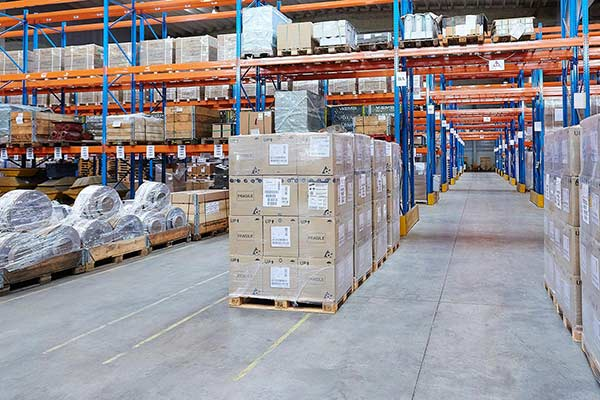
\includegraphics[width = \textwidth]{images/logisticsolutions.jpg}
    \end{column}
\end{columns}
\end{frame}

\begin{frame}{GobotSim, a new factory simulator with an emphasis on deliberation}
    \begin{columns}
        \begin{column}{0.5\textwidth}
            GobotSim, a 2D factory simulator to study scheduling and resource allocation strategies.
        \end{column}
        \begin{column}{0.4\textwidth}
            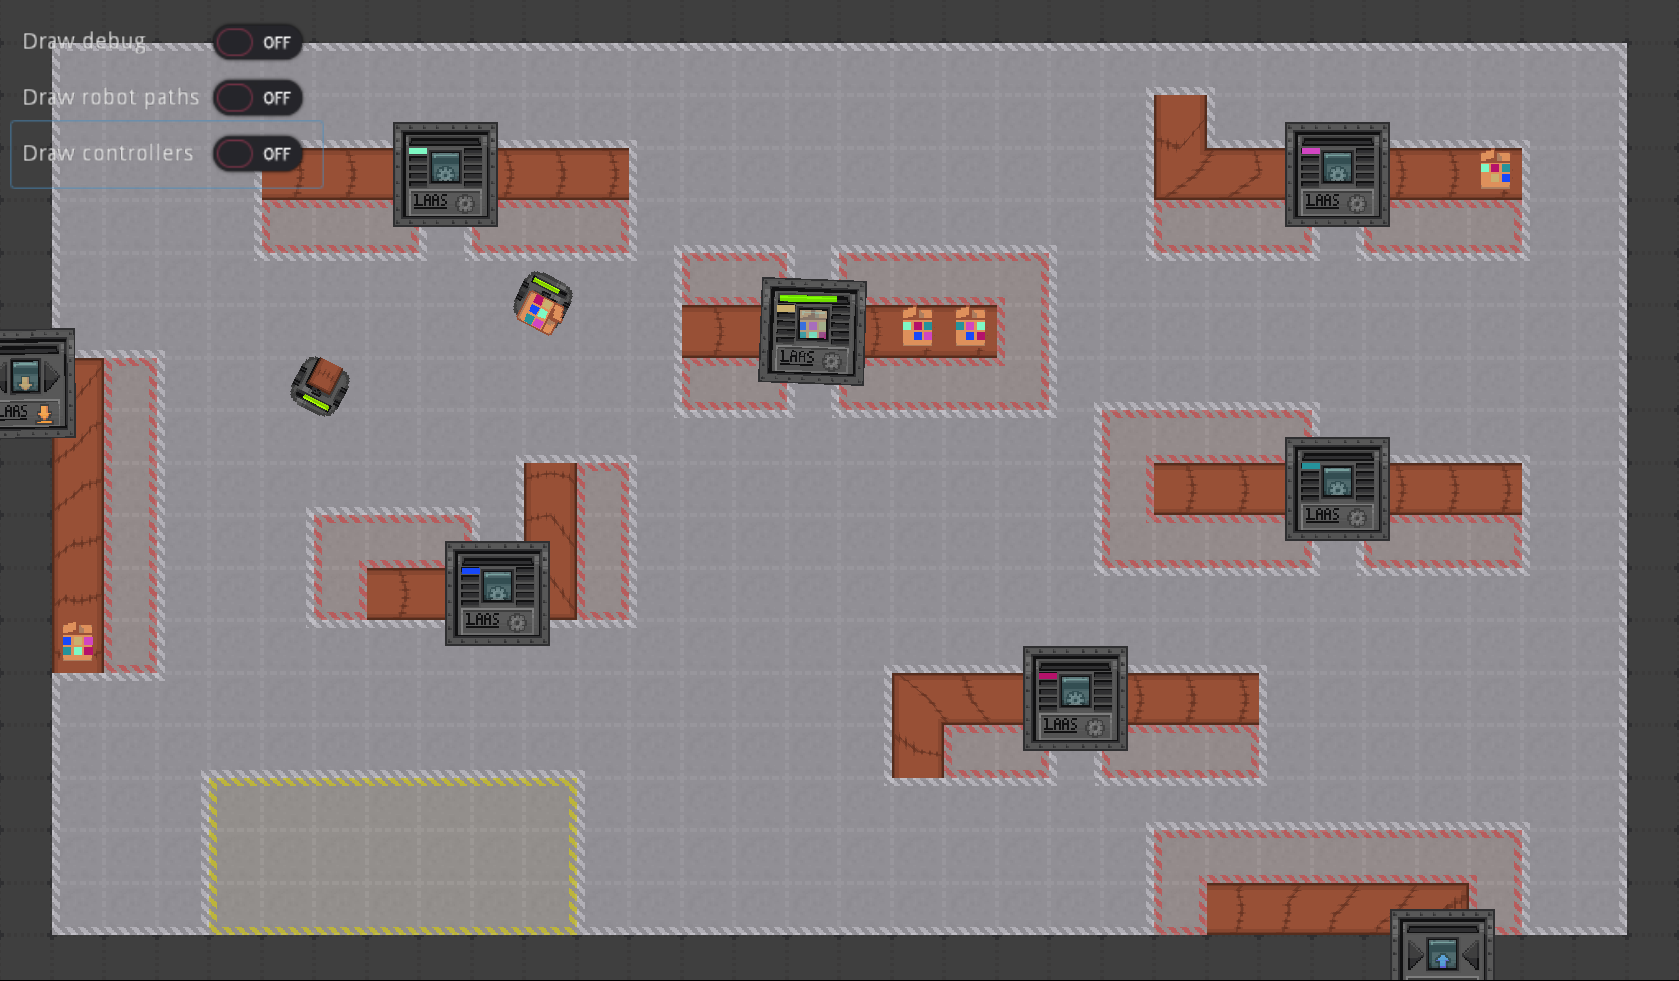
\includegraphics[width=\linewidth]{images/gobot-rae.png}
        \end{column}
    \end{columns}
    
    ~~


    \centering
    \emph{Environment}

~~


    \begin{columns}
        \begin{column}{0.3\textwidth}
            \centering
            Package

            
\includegraphics[width = 0.5\textwidth]{images/godot/package.png}
        \end{column}
        \begin{column}{0.3\textwidth}
            \centering
            Machine

            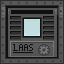
\includegraphics[width = 0.5\textwidth]{images/godot/machine_texture.png}

        \end{column}
        \begin{column}{0.3\textwidth}
            \centering
            Robot

            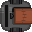
\includegraphics[width = 0.5\textwidth]{images/godot/robot_texture.png}
        \end{column}
    \end{columns}

    % \begin{columns}
    %     \begin{column}{0.2\textwidth}
            
    %     \end{column}
    %     \begin{column}{0.7\textwidth}
    %         Machines
    %         \begin{itemize}
    %             \item Processing : does a predefined list of process for packages
    %             \item Input: generate packages
    %             \item Output: gather fully processed packages
    %         \end{itemize}
    %     \end{column}
    % \end{columns}

    % ~

    % \begin{columns}
    %     \begin{column}{0.2\textwidth}
            
    %     \end{column}
    %     \begin{column}{0.7\textwidth}
    %         Robots : manipulate packages
    %         \begin{itemize}
    %             \item commands: move, pick, place,\dots
    %             \item recharge at recharge areas
    %         \end{itemize}
    %     \end{column}
    % \end{columns}
\end{frame}

% \begin{frame}{Other logistic simulators}
%     \begin{columns}[t]
%         \begin{column}{0.5\textwidth}
%             \small
%             Robocup Logistic League Simulation \cite{niemuellerPlanningCompetitionLogistics2016}

%             \includegraphics[width = \linewidth]{images/robocup.png}
            
%         \end{column}
%         \begin{column}{0.5\textwidth}
%             \small
%             CraftBots \cite{nemiroDesigningAdaptableBenchmark2021}

%             \includegraphics[width = \linewidth]{images/craftbots.png}
%         \end{column}
%     \end{columns}
    
% \end{frame}

\begin{frame}{Mission of the robotic agent}
Mission : Do all the processes of packages.
For each process of a package:
\begin{itemize}
    \item Select a machine to do the process.
    \item Select a robot to carry it to the machine.
\end{itemize}
% ~

%     Role of the autonomous agent:
%     \begin{itemize}
%         \item Control individual AMR.
%         \item Deal with contingencies and errors,
%         \item Optimize choices in function of time and energy.
%     \end{itemize}
\end{frame}
\subsection{Programming the autonomous agent}

\begin{frame}{Programming the autonomous agent}
    Hierarchical representation of the agent skills.
    \begin{itemize}
        \item Different methods for adapted to various contexts.
        \item Different levels of modelling and abstraction $\rightarrow$ ease deliberation.
    \end{itemize}
   
\end{frame}

\begin{frame}{Procedure based system}
    Refinement-based acting with the Refinement Acting Engine (RAE) \cite{ghallabAutomatedPlanningActing2016}:
    \begin{itemize}
        \item Procedure-based system.
        \item Monitor procedure and command execution
        \item Support parallel execution.
        \item Refinement at runtime for more reactive systems.
        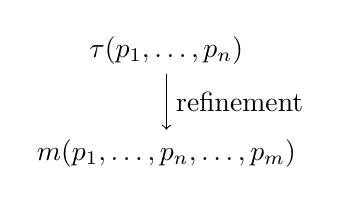
\begin{tikzpicture}
            \node[] (task) {$\tau(p_1,\dots,p_n)$};
            \node[below = 2em of task] (method) {$m(p_1,\dots,p_n, \dots, p_m)$};
            \path[->] (task) edge node[right, midway] {refinement} (method);
        \end{tikzpicture}
    \end{itemize}
\end{frame}

\begin{frame}{Hierarchical operational models to represent the capabilities of an agent}

\begin{columns}[T]
    \begin{column}{0.55\textwidth}
        Agent behavior = collection of skills (procedures)
        
        ~
        \pause
        Hierarchical operational models : Acting domain \textbf{$A_\Delta (A, T, M_t)$}
        \small
        \pause
        \begin{itemize}
        
        
         \item[$A$] : commands (low-level) move, grasp
         \pause
         \item[$T$] : tasks (high-level)
         \pause
         \item[$M_t$] : methods: pre-conditions, body (operational model)
         
     \end{itemize}
    \end{column}
    \pause
    \begin{column}{0.45\textwidth}
        \begin{figure}
            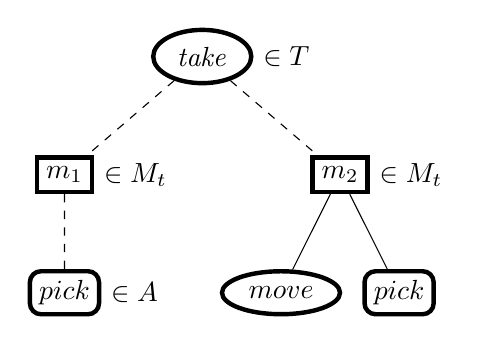
\begin{tikzpicture}
                \node[draw, ellipse, ultra thick] (t) {\textit{take}} [sibling distance = 3.5cm]
                  child {node[draw, ultra thick] (m1) {$m_1$} edge from parent [dashed]
                  child {node[draw,rounded corners, ultra thick, solid] (a1) {$pick$} edge from parent
                  }} 
                  child {node[draw, ultra thick] (m2) {$m_2$} edge from parent [dashed] [sibling distance = 1.5cm]
                  child {node[draw, ellipse, ultra thick, solid] (a2) {$move$} edge from parent [solid]}
                  child {node[draw, rounded corners, solid, ultra thick] {$pick$} edge from parent [solid]}};
                \node[right = 0em of t] {$\in T$};
                \node[right = 0em of m1] {$\in M_t$};
                \node[right = 0em of m2] {$\in M_t$};
                \node[right = 0em of a1] {$\in A$};

            \end{tikzpicture}
            \caption{Example of hierarchy for the \textit{task} \textit{open door}}

            
        \end{figure}
    \end{column}
\end{columns}
    
\end{frame}

\begin{frame}{RAE algorithms}
    \begin{columns}[T]
  
        \begin{column}{0.65\textwidth}
            
            Algorithms:
            \small
            \begin{itemize}
                \setlength{\leftmargini}{-1pt}
                \onslide<2->
                \item \textbf{Main:} 
                \begin{itemize}
                    \item Receive $\tau$ (task or event);
                    
                    add it to the \textbf{agenda} (ongoing tasks)
                    \onslide<3->
                    \item Refine $\tau$: \textbf{Select} an applicable method $m$ for $\tau$
                    \onslide<4->
                    \item \textbf{Progress} $m$
                \end{itemize}
                \onslide<5->
                \item \textbf{Progress:}
                    \begin{itemize}
                        \onslide<6->
                        \item Monitor execution of $m$.
                        \onslide<7->
                        \item Refine subtasks in $m$.    
                        \onslide<8->
                        \item Monitor execution of subtasks.
                        \onslide<9->
                        \item \textbf{Retry} $\tau$ in case of \emph{failure}:
                    
                    Call \textbf{Select} to get a new method;
                    
                    \textbf{Progress} the new method.
                    \end{itemize}
            \end{itemize}
        \end{column}
        \begin{column}{0.35\textwidth}
            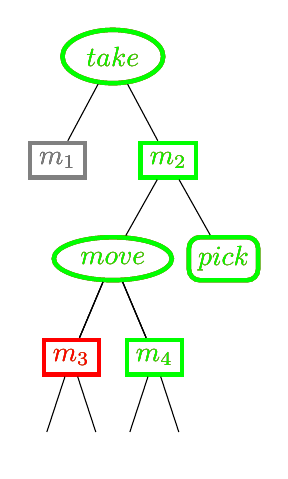
\begin{tikzpicture}
                \onslide<2>
                \node[draw,ellipse, ultra thick] (t) {$take$};
                \onslide<3-9>
                \node[draw,ellipse, ultra thick, color = orange] (t) {$take$};
                \onslide<10>
                \node[draw,ellipse, ultra thick, color = green] (t) {$take$};
                \onslide<3>
                \node[draw, ultra thick, below= 2em of t, xshift = -2em] (m1) {$m_1$};
                \node[draw, ultra thick, below= 2em of t, xshift = 2em] (m2) {$m_2$};
                \onslide<4->
                \node[draw, ultra thick, below= 2em of t, xshift = -2em, color = gray] (m1) {$m_1$};
                \node[draw, ultra thick, below= 2em of t, xshift = 2em, color = orange] (m2) {$m_2$};
                \onslide<10>
                \node[draw, ultra thick, below= 2em of t, xshift = 2em, color = green] (m2) {$m_2$};
                \onslide<3->
                \path[-] (t) edge (m1) (t) edge (m2);
                \onslide<5>
                \node[draw,rounded corners, ultra thick, solid, below = 2em of m2, xshift = 2em] (a1) {$pick$};
                \onslide<6>
                \node[draw,rounded corners, ultra thick, solid, below = 2em of m2, xshift = 2em, color = orange] (a1) {$pick$};
                \onslide<7->
                \node[draw,rounded corners, ultra thick, solid, below = 2em of m2, xshift = 2em, color = green] (a1) {$pick$};
                \onslide<5-7>
                \node[draw,ellipse, ultra thick, solid, below = 2em of m2, xshift = -2em] (t2) {$move$};
                \onslide<8->
                \node[draw,ellipse, ultra thick, solid, below = 2em of m2, xshift = -2em, color = orange] (t2) {$move$};
                \onslide<10>
                \node[draw,ellipse, ultra thick, solid, below = 2em of m2, xshift = -2em, color = green] (t2) {$move$};
  
  
                \onslide<5->
                \path[-] (m2) edge (a1) (m2) edge(t2);
  
  
                \onslide<7>
                \node[draw, ultra thick, below = 2em of t2, xshift = -1.5em] (m3) {$m_3$};
                \node[draw, ultra thick, below = 2em of t2, xshift = 1.5em] (m4) {$m_4$};
                \path[-] (t2) edge  (m3) (t2) edge (m4);
                
                \onslide<8>
                \node[draw, ultra thick, below = 2em of t2, xshift = -1.5em, color = orange] (m3) {$m_3$};
                \node[draw, ultra thick, below = 2em of t2, xshift = 1.5em, color = gray] (m4) {$m_4$};
                \path[-] (t2) edge  (m3) (t2) edge (m4);
  
                \onslide<9->
                \node[draw, ultra thick, below = 2em of t2, xshift = -1.5em, color = red] (m3) {$m_3$};
                \node[draw, ultra thick, below = 2em of t2, xshift = 1.5em, color = orange] (m4) {$m_4$};
                \path[-] (t2) edge  (m3) (t2) edge (m4);
                \onslide<10>
                \node[draw, ultra thick, below = 2em of t2, xshift = 1.5em, color = green] (m4) {$m_4$};
                
                \onslide<8->
                \node[below = 2em of m3, xshift = -1em] (e3) {};
                \node[below = 2em of m3, xshift = 1em] (e4) {};
                \path[-] (m3) edge  (e3) (m3) edge (e4);
  
                \onslide<8->
                \node[below = 2em of m4, xshift = -1em] (e5) {};
                \node[below = 2em of m4, xshift = 1em] (e6) {};
                \path[-] (m4) edge  (e5) (m4) edge (e6);
      
            \end{tikzpicture}
        \end{column}
    \end{columns}    
\end{frame}



\begin{frame}[fragile]{Simple scenario: one package}
    \centering
    \begin{columns}
        \begin{column}{0.5\textwidth}
            \centering
            
\includegraphics[width = 0.3\textwidth]{images/godot/package.png}
            
            \LARGE \emph{$\times 1$}
        \end{column}
        \begin{column}{0.5\textwidth}
            \centering
            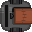
\includegraphics[width = 0.3\textwidth]{images/godot/robot_texture.png}
            
            \LARGE \emph{$\times 1$}
        \end{column}
    \end{columns}
    \pause
    \begin{itemize}
        \item task: process(?p)
        \item methods:
    \end{itemize}
    \footnotesize
    \begin{columns}[t]
        \begin{column}{0.32\textwidth}
            m1(?p, ?r, ?m)
            \begin{align*}
                pre: &\ proc(?p) \neq \emptyset \\
                 &battery(?r) > 40\% \\
                 &proc(?p)[1] \in proc(?m) \\
                 body:&take(?p,?r) \\
                     &carry(?p,?r,?m) \\
                     &process(?p)
            \end{align*}
        \end{column}
        \begin{column}{0.32\textwidth}
            m2(?p, ?r, ?m)
            \begin{align*}
                pre: &\ proc(?p)  = \emptyset \\
                 &battery(?r) > 40\% \\
                 &kind(?m) = \text{output} \\
                 body:&take(?p,?r) \\
                     &carry(?p,?r,?m) \\
            \end{align*}
        \end{column}
        \begin{column}{0.32\textwidth}
            m3(?p, ?r) 
            \begin{align*}  
                pre: &battery(?r) \leq 40\% \\
                 body:&recharge(?r) \\
                     &process(?p)
            \end{align*}
        \end{column}
    \end{columns}
    % \begin{align*}
    %     \text{task:} & \text{process(?p)}\\
    %     \text{methods:}& \\
    %     m1(?p, ?r, ?m) \\
    %     \text{pre:} & !empty(processes(?p)) \\
    %      &battery(?r) \leq 40\% \\
    %      &first(processes(?p)) \in processes(?m) \\
    %      body:&take(?p,?r) \\
    %          &carry(?p,?r,?m) \\
    %          &process(?p)
    % \end{align*}
    
\end{frame}

\begin{frame}{Running example with one package}
    \LARGE
    \centering
    \href{https://youtu.be/a4_tITUTQuQ}{Video example}
\end{frame}

\subsection{Multi-agent scenario}

\begin{frame}{Several packages?}
    \begin{columns}
        \begin{column}{0.5\textwidth}
            \centering
            
\includegraphics[width = 0.5\textwidth]{images/godot/package.png}
            
            \Large $\times n$
        \end{column}
        \begin{column}{0.5\textwidth}
            \centering
            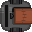
\includegraphics[width = 0.5\textwidth]{images/godot/robot_texture.png}
            
            \LARGE $\times m$
        \end{column}
    \end{columns}
    
    ~

    New decisions for the robotic system:
    \begin{itemize}
        \item Schedule package passage on machines
        \item Allocate package displacement tasks to robots
        %\item Monitor the robots' batteries 
    \end{itemize}

    \centering
\end{frame}

\begin{frame}{Multi-agent refinement-based deliberation}
    \begin{columns}[t]
        \begin{column}{0.45\textwidth}
            RAE shortcomings:
            \begin{itemize}
                \item Progression of tasks relies on Round Robin
                \item Methods limited to a sequence of actions
                %\item Difficulties to integrate sound planning from operational models due to implementation in Python.
            \end{itemize}
        \end{column}
        \begin{column}{0.1\textwidth}
            $\rightarrow$

        \end{column}
        \begin{column}{0.45\textwidth}
            Adapt RAE for multi-agents to
            \begin{itemize}
                \item Deal with concurrency
                \item Improve the interleaving of parallel tasks
                \item Reason on shared resources to optimize the overall process
            \end{itemize}
        \end{column}
    \end{columns}
\end{frame}
%\section{Deliberative agent (7 min)}

\begin{frame}{What is an agent}

    \begin{columns}[T]
        \begin{column}{0.3\textwidth}
            A robotic agent

            ~

            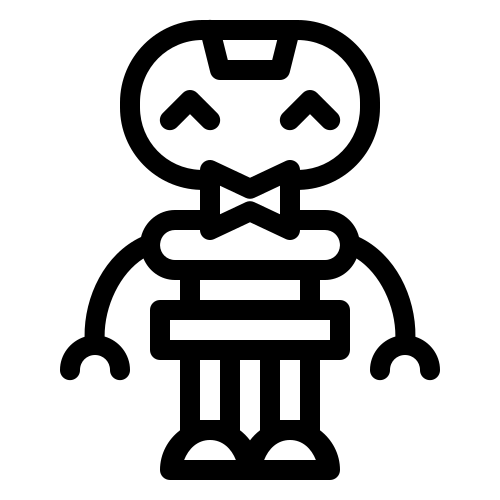
\includegraphics[width = 0.7\textwidth]{images/icons8-robot-gustav-500.png}
        \end{column}
        \begin{column}{0.7\textwidth}
            \center capable of :
            \pause
            \begin{enumerate}
                \item Perceiving its environment
                \pause
                \item Modifying its environment (actions)
                \pause
                \item \textbf{Deliberating:} Reasoning about its \textbf{skills} in order to fulfill a goal
            \end{enumerate}
        \end{column}
    \end{columns}

 
\end{frame}

\begin{frame}{Represent the skills of an agent}

\begin{columns}[T]
    \begin{column}{0.6\textwidth}

        Robot behavior = \textbf{operational model}:
        \begin{itemize}
            \item Executable program
            \item General purpose language
        \end{itemize}
        
        ~

        
        Acting domain \textbf{$A_\Delta (A, T, M_t)$}: Hierarchical operational models
        
                \begin{itemize}
        
        
         \item[$A$] \textit{(low-level skills)}: primitive tasks
         \pause
         
         \textit{\footnotesize(move, grasp, look)}
         \pause
         \item[$T$] \textit{(high-level skills)}: abstract tasks
         \pause

         \textit{\footnotesize(set the table, prepare a coffee)}
         \pause
         \item[$M_t$] \textit{("Know how")}: methods (operational models)

         
     \end{itemize}
    \end{column}
    \begin{column}{0.45\textwidth}
        \begin{figure}
            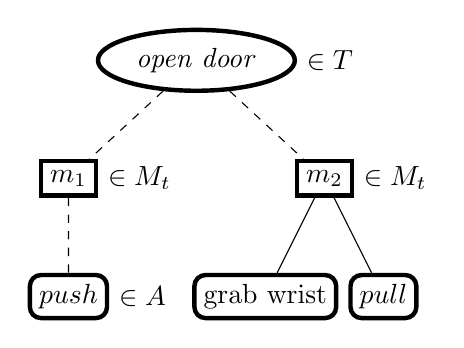
\begin{tikzpicture}
                \node[draw,ellipse, ultra thick] (t) {\textit{open door}} [sibling distance = 3.25cm]
                  child {node[draw, ultra thick] (m1) {$m_1$} edge from parent [dashed]
                  child {node[draw,rounded corners, ultra thick, solid] (a1) {$push$} edge from parent
                  }} 
                  child {node[draw, ultra thick] (m2) {$m_2$} edge from parent [dashed] [sibling distance = 1.5cm]
                  child {node[draw, rounded corners, solid, ultra thick] (a2) {grab wrist} edge from parent [solid]}
                  child {node[draw, rounded corners, solid, ultra thick] {$pull$} edge from parent [solid]}};
                \node[right = 0em of t] {$\in T$};
                \node[right = 0em of m1] {$\in M_t$};
                \node[right = 0em of m2] {$\in M_t$};
                \node[right = 0em of a1] {$\in A$};

            \end{tikzpicture}
            \caption{Example of hierarchy for the \textit{task} \textit{open door}}

            
        \end{figure}
    \end{column}
\end{columns}
    
\end{frame}
\begin{frame}{Refinement Acting Engine (RAE)\cite{ghallabAutomatedPlanningActing2016} : Deliberation algorithms using hierarchical operational models}
\begin{columns}
    \begin{column}{0.35\textwidth}
    \pause
    \setlength{\leftmargini}{-1pt}
    %\setlength{\parsep}{1pt}
    %\setlength{\parskip}{0pt}
    RAE features:
    \small
    \begin{itemize}
        \item Perform multiple tasks in parallel
        \pause
        \item Automated deliberation: Refinement of task
        \begin{itemize}
            \setlength{\leftmargini}{-1pt}
            \pause
            \item Refinement of task into a method
            \pause
            \item Instantiating of \textbf{arbitrary} variables
        \end{itemize}
    \end{itemize}
    \end{column}
    \begin{column}{0.65\textwidth}
        Algorithms:
        \small
        \begin{itemize}
            \setlength{\leftmargini}{-1pt}
            \item \textbf{Main:} 
            \begin{itemize}
                \item Receive $\tau$ (task or event);
                
                add it to the \textbf{agenda} (ongoing tasks)
                \pause
                \item Refine $tau$: \textbf{Select} an applicable method $m$ for $\tau$
                \pause
                \item \textbf{Progress} $m$
            \end{itemize}
            \item \textbf{Progress:}
                \begin{itemize}
                \item Monitor execution of $m$.
                \item Refine subtasks in $m$.    
                \item Monitor execution of subtasks.
                \item \textbf{Retry} $\tau$ in case of \emph{failure}:
                
                Call \textbf{Select} to get a new method;
                
                \textbf{Progress} the new method.
                \end{itemize}
                \pause
        \end{itemize}
    \end{column}
\end{columns}

    
\end{frame}

\begin{frame}{Improve the refinement using planning}
    \begin{center}
        
    Role of Select:

    ~

    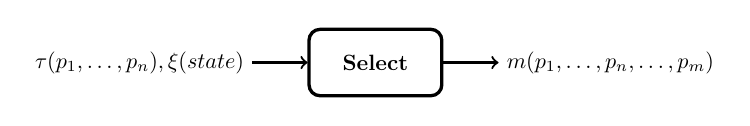
\begin{tikzpicture}[thick,scale=0.8, every node/.style={scale=0.8}]
    \node[draw = black, very thick,
        minimum width = 6em,
        minimum height = 3em,
        rounded corners,
        text = black,
        align=center,] (F) at (0,0) {\textbf{Select}};
        
    \pause
    \node[left= 2em of F] (i) {\textbf{$\tau(p_1,\dots,p_n), \xi (state)$}};
    \node[right= 2em of F] (o) {\textbf{$m(p_1, \dots, p_n,\dots,p_m)$}};
    \pause
    \path[->]
    (i) edge (F)
    (F) edge (o);

    \end{tikzpicture}
    

    %$Select(\tau, p_1,\dots,p_n) \rightarrow \{m_s, p_1, \dots, p_n,\dots,p_m\}$

    \end{center}

    Techniques:
    \begin{itemize}

    \item Greedy (Basic RAE functioning): arbitrary applicable method
    \pause
    
    \underline{Problem:} Does not take into account future refinements (can lead into dead-locks)
    \pause
    \item \textbf{look-ahead(planning)} : capacity to project the system from the current state to possible future state

    \end{itemize}
\end{frame}
\begin{frame}{How to use planning in RAE}
    %Make a high-level choice based on future choices the agent will have to make and its own capabilities to modify its environment.
    Requires:
    \begin{itemize}
        \item A planner
        \item Descriptive model of the agent skills : describes the set of states that may result from performing tasks.
    \end{itemize} 

    Descriptive models shortcomings:
    \begin{itemize}
        \item Made limited dedicated languages: PDDL \cite{foxPDDL2ExtensionPDDL2003}, ANML \cite{smith2008anml},\dots
        \item operational model $\not\equiv$ descriptive model $\rightarrow$ Harder design
    \end{itemize}

    ~
    
    \centering
    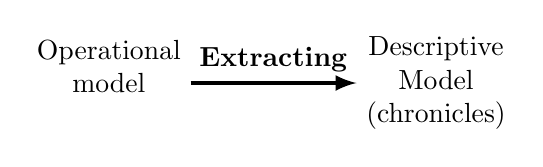
\begin{tikzpicture}
        \node[align = center] (O) {Operational\\ model \\};
        \node[right=6em of O, align = center] (D) {Descriptive\\ Model \\(chronicles)};
        \draw[-latex, ultra thick] (O.east)-- node[above, midway] (c) {\textbf{Extracting}} (D.west);
    \end{tikzpicture}

    Plan with \textbf{Aries} (hierarchical LCP\cite{bit-monnotConstraintBasedEncodingDomainIndependent2018} extension):

\end{frame}

\begin{frame}[c]{An analyzable acting language to extract descriptive models}
    \begin{columns}[c]
        \begin{column}{0.45\textwidth}
            Acting language Requirements:
            \begin{itemize}
                \item General purpose language
                \item Identified and simple semantic
            \end{itemize}
        \end{column}
        \begin{column}[c]{0.1\textwidth}
            \centering
            $\rightarrow$
        \end{column}
        \begin{column}{0.5\textwidth}
            Lisp dialect (Scheme variant) \cite{moretti1979lambda}

            Perks:
            \begin{itemize}
                \item Few primitives
                \item Immutable
                \item Functional
                \item Pure
            \end{itemize}
        \end{column}
    \end{columns}
\end{frame}

\begin{frame}{Synthesis of the proposition}
    \pause
        \centering
        Task refinement guided by planning:

        ~
        
        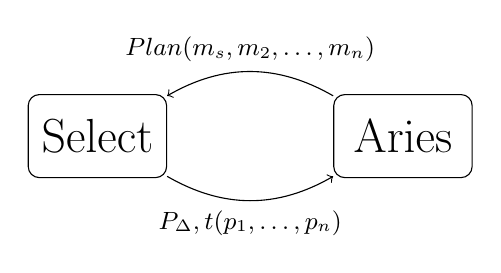
\begin{tikzpicture}
            \node[draw,
            rounded corners,
            minimum width = 5em,
            minimum height = 3em] (select) {\LARGE Select};
            \node[draw,
            rounded corners,
            right = 6em of select,
            minimum width = 5em,
            minimum height = 3em] (aries) {\LARGE Aries};
            \path[->, every node/.style={font=\sffamily\small}]
            (select) edge[bend right] node [right, below] {$P_\Delta, t(p_1,\dots,p_n)$} (aries)
            (aries) edge[bend right] node [right, above] {$Plan(m_s, m_2,\dots,m_n)$} (select)
            ;
        \end{tikzpicture}

        ~
    
        Planning domain extraction from operational models:

        ~

        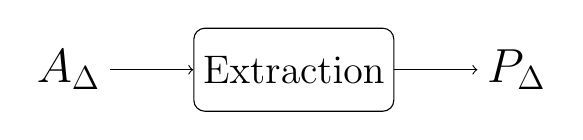
\begin{tikzpicture}
            \node (acting) {\LARGE $A_\Delta$};
            
            \node[draw,
            rounded corners,
            right= 3em of acting,
            minimum height = 3em,
            minimum width = 6em] (ext) {\Large Extraction};
        
            \node[right = 3em of ext] (planning) {\LARGE $P_\Delta$ };
            
            \path[->, every node/.style={font=\sffamily\small}]
            (acting) edge (ext)
            (ext) edge (planning);
          \end{tikzpicture}

\end{frame}



%\section{RAE for multi-agent systems}
\subsection{Operational Model Planning and Acting System}

\begin{frame}{The Operational Model Planning and Acting System (OMPAS), an extension to RAE}
    \begin{columns}[t]
        \begin{column}{0.5\textwidth}
    New \textbf{task} in \textbf{dedicated thread}
    \begin{figure}
        \tikzstyle{thread} = [draw, rounded corners, rectangle, fill=black!50]
    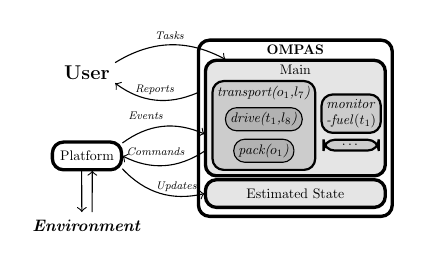
\begin{tikzpicture}[scale=0.5, every node/.style={scale=0.5}]
  
        %RAE
        \node[draw = black, very thick,
            minimum width = 14em,
            minimum height = 5em,
            rounded corners,
            text = black,
            text centered, text depth = 4 cm,
            align = center,
            ] (R) at (0,0) {\textbf{OMPAS}};
        %Operational Models
        % \node[draw = black, ellipse, very thick,
        %     minimum width = 7em,
        %     minimum height = 2em,
        %     above = 1em of R,
        %     text = black,
        %     text centered, align=center
        % ] (OM) {\textit{Operational Models} %($A_\Delta$)
        % };
  
  
        %state
        \node[draw = black, very thick,
        text centered,
        minimum width = 13em,
        minimum height = 2em,
        rounded corners,
        text = black,
        fill=black!10,
        align = center] (S) at ($(R.south) + (0,0.6)$) {Estimated State};
  
        %main
        \node[draw = black, very thick,
        minimum height = 8em,
        minimum width = 13em,
        rounded corners,
        text = black,
        text centered, text depth = 7em,
        fill=black!10,
        align=center] (main) at ($(R.north) + (0,-2)$) {Main};
  
        %t1
        \node[draw = black, thick,
        minimum height = 6em,
        minimum width = 7em,
        rounded corners,
        text = black,
        text centered, text depth = 5em,
        fill=black!20,
        align=center](t1) at ($(main.south) + (-0.8, 1.3)$) {\emph{transport($o_1$,$l_7$)}};
  
  
        %first task
        \node[draw, rounded corners, rectangle, fill=black!30] (st11) at ($(t1.south) + (0,1.3)$) {\emph{drive($t_1$,$l_8$)}};
        \node[draw, rounded corners, rectangle, fill=black!30] (st12) at ($(st11.south) + (0,-.5)$){\emph{pack($o_1$)}};
        
        \node[draw, thick, rounded corners, rectangle,minimum width = 4em, fill=black!20, align= center] (t3) at ($(t1.east) + (0.9, 0.3)$){\textit{monitor}\\
        \textit{-fuel}($t_1$)};
        \node[draw, thick, rounded corners, rectangle,minimum width = 4em, fill=black!20, align= center] (t3) at ($(t1.east) + (0.9, -0.5)$){\dots};
  
  
  
        %platform
        \node[draw = black, very thick,
        text centered,
        minimum width = 5em,
        minimum height = 2em,
        %below = 2em of R,
        rounded corners,
        text = black,
        align = center,] (Pl) at ($(R.west) +(-8em, -2em)$) {Platform};
  
        \node[text centered,
        minimum width = 5em,
        minimum height = 2em,
        below = 1.5em of Pl,
        rounded corners,
        text = black,
        align = center,] (E) {\textbf{\large\textit{Environment}}};
  
        \node[very thick,
            text centered,
            rounded corners,
            text = black] (U) at ($(R.west) +(-8em, +4em)$) {\Large \textbf{User}};
        
        % \node[draw = black, very thick,
        %     text centered,
        %     right = 7em of R,
        %     minimum width = 5em,
        %     minimum height = 4em,
        %     rounded corners,
        %     text = black] (Pl) {Platform};
        
  
        \path[->]
  
            %Link between operational models library
            %(OM) edge (R)
  
            (U.20) edge[bend left] node [midway, above, align=center] {\footnotesize \emph{Tasks}} (main.+140)
            (R.+160) edge [bend left] node [midway, above] {\footnotesize \emph{Reports}} (U.-20)
        
            %Link between RAE and the platform
            (main.-160) edge[bend left] node [pos = 0.6, above = 0.2em] {\footnotesize \emph{Commands}} (Pl.east)
            
            %between platform and state
            (Pl.-20) edge [bend right] node [pos = 0.7, right, above, align = center] {\footnotesize \emph{Updates}} (S.west)
            
            %between platform and main
            (Pl.20) edge [bend left] node [pos = 0.3, right, above= 0.2em, align = center] {\footnotesize \emph{Events}} (main.-170)
  
            (Pl.-110) edge (E.110)
            (E.70) edge (Pl.-70)
            ;
        
        \end{tikzpicture}
        \caption{Overview of OMPAS architecture}
    \end{figure}
            
        \end{column}
        \pause
        \begin{column}{0.5\textwidth}
        Operational language with
        \begin{itemize}
            \item \textbf{Acting} features
            \item \textbf{Generic} programming constructs
            \item First-hand concurrency support (interruption, resource)
            \item \textbf{Simple semantic} $\rightarrow$ \textbf{guide} the \textbf{acting choices} with \textbf{automated analysis} of \textbf{skills}
        \end{itemize}
        \end{column}
    \end{columns}
\end{frame}

\subsection{Acting language}

\begin{frame}[fragile]{SOMPAS: A Lisp variant based on Scheme}
    \centering
    Scheme : Recursive evaluation of \textbf{expressions} \verb|(f e1 ... en)|
    
    ~~

\pause
    \begin{columns}[t]
        \begin{column}{0.65\textwidth}
            Definitions:
            \begin{itemize}
                \item \textbf{Expression} = \{Atom, List of expression\}
                \item \textbf{Atom} = \{Symbol, Boolean, Number, Procedure\}
            \end{itemize}
\pause
        \end{column}
        \begin{column}{0.35\textwidth}
            Scheme \textbf{advantages}:
            \begin{itemize}
                \item Few primitives
                \item Functional
                \item \textbf{Simple to extend}
            \end{itemize}
        \end{column}
     \end{columns}
\end{frame}

\begin{frame}[fragile]{Acting primitives}
    \begin{columns}
        \begin{column}{0.5\textwidth}
            Functions:
            \begin{itemize}
                \pause
                    \item \textbf{\textit{(exec a $p_1...p_n$)}} executes and monitors a task or command.
                    % \begin{itemize}
                    %     \item command : resorts to the platform
                    %     \item task: selects a method and execute its operational model.
                    % \end{itemize}
                \pause
                    \item \textbf{\textit{(read-state sf $p_1...p_n$)}} returns the value of a state-variable
                % \pause
                %     \item \textit{(arbitrary set $\lambda$)} returns an arbitrary element from a $set$%. $\lambda$ can be used to select among the $set$.
                \end{itemize}
        \end{column}
    \pause
        \begin{column}{0.5\textwidth}
               
        Example:
    \small
        \lstset{columns=fullflexible}
        \begin{lstlisting}[language = lisp]
    (begin
        (define loc-p (read-state loc ?p))
        (define loc-r (read-state loc ?r))
        (if (!= loc-p loc-r)
            (exec move ?r loc-p))
        (exec pick ?r ?p) 
        (exec move ?r ?l)
        (exec place ?r ?p))             
        \end{lstlisting}
        \end{column}
    \end{columns}
    \end{frame}


\begin{frame}[fragile]{Scheme extension for concurrency and interruption}

    Definition of a new Atom: the \emph{handle}
    
    ~~
\pause
    \begin{columns}
        \begin{column}{0.6\textwidth}
            Functions:
            \begin{itemize}
                \item \textbf{\textit{(async e)}}: creates a new thread to evaluate e, returns a handle
                \item \textbf{\textit{(await h)}}: awaits the result of the concurrent evaluation.
                \item \textbf{\textit{(interrupt h)}}: interrupts the concurrent evaluation.
                \item \textbf{\textit{(uninterruptible e)}}: prevent interruption signals.
            \end{itemize}
        \end{column}
        \pause
        \begin{column}{0.4\textwidth}
        Example: 
\small
\lstset{columns=fullflexible}
            \begin{lstlisting}[language = lisp]
(begin
    (define h1 (async (+ 1 2)))
    (define h2 (async (* 3 3)))
    (+ (await h1) (await h2)))
-> 12 
            \end{lstlisting}
        \end{column}
    \end{columns}
\end{frame}

\begin{frame}[fragile]{Example of program with interruptions.}
    
\begin{columns}
    \begin{column}{0.4\textwidth}
        \lstset{basicstyle=\footnotesize, columns=fullflexible}
\begin{lstlisting}[language=lisp]
(begin
 (define h
  (async 
    (begin
     (uninterruptible (begin
       (exec pick ?r ?o)
       (exec move ?r ?l)
       (exec drop ?r ?o)))
     (exec inspect ?r ?o))))
 (race 
   (await h)
   (begin
    (sleep 10)
    (interrupt h))))
\end{lstlisting}

    \end{column}
    \begin{column}{0.6\textwidth}
        \newcommand{\Cross}{$\mathbin{\tikz [x=1.4em,y=1.4em,line width=.2em, red] \draw (0,0) -- (1,1) (0,1) -- (1,0);}$}
    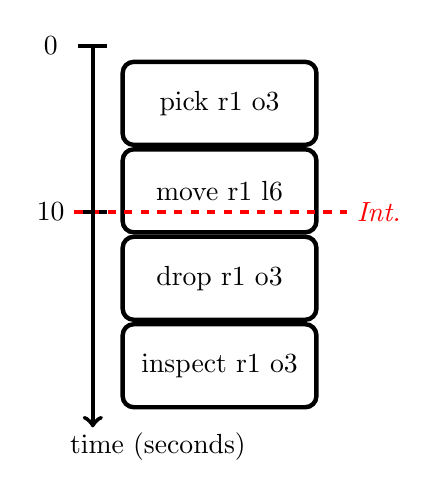
\begin{tikzpicture}
        \node[draw,
        rounded corners,
        ultra thick,
        minimum height = 3em,
            minimum width = 7em,] (pick) at (0,0) {pick r1 o3};
    
        \node[draw, rounded corners,
        ultra thick,
            minimum height = 3em,
            minimum width = 7em,
        ] (move) at ($1.5*(pick.south)-0.5*(pick.north)$) {move r1 l6};
        %\action{move, move r1 l6, 10em, pick}
    
        \node[draw, rounded corners,
        ultra thick,
            minimum height = 3em,
            minimum width = 7em,
        ] (drop) at ($1.5*(move.south) - 0.5*(move.north)$) {drop r1 o3};
        \node[draw, rounded corners,
        ultra thick,
            minimum height = 3em,
            minimum width = 7em,
        ] (inspect) at ($1.5*(drop.south) - 0.5*(drop.north)$) {inspect r1 o3};
        \node at (inspect) {\Cross};
    
            \node[] (origin) at ($(pick.north west) + (-1em,+0.5em)$) {~~};
        
            \node[] (zero) at ($(origin.west) + (-1em,0)$) {0};
            \draw[-, ultra thick] (origin.west) -- (origin.east);
            \node[] (ten) at ($(zero) + (0,-6em)$) {10};
            \draw[-, ultra thick] ($(origin.west) + (0,-6em)$) -- ($(origin.east) + (0,-6em)$);
    
    
            \node[] (interruption) at ($(ten.east) +(11em,0em)$){\color{red} \textit{Int.}};%{\color{red} \textit{interruption}};
            \draw[-, ultra thick, dashed, color= red] ($(ten.east)$) -- ( interruption);
            \node[] (end) at ($1.5*(inspect.south west) - 0.5*(inspect.south west) + (-1em,-1em)$) {};
            \node[] (time) at ($1.5*(end.south east) - 0.5*(end.south east) + (2em,0)$)  {time (seconds)};
    
    
        \path[->] (origin.center) edge[ultra thick] (end);
    \end{tikzpicture}
    \end{column}
\end{columns}    
\end{frame}


\begin{frame}[fragile]{Resource model for safe concurrent execution}
    Definition of a resource:
    \begin{columns}
        \begin{column}{0.5\textwidth}
            \begin{itemize}
                \item Object \textbf{r} with initial capacity $C(0) = C_{init} $
                \item Acquire($r$,$c$) at time $t$ $\implies$ $c \leq C(t)$ 
            \end{itemize}
        \end{column}
        \pause
        \begin{column}{0.5\textwidth}
            \begin{itemize}
                \item \textbf{\textit{unary}:} $C_{init} = 1, c = 1$;
                \item \textbf{\textit{divisible}}: $C_{init} \in  \mathbb{R}_+^*, c \in ]0, C(t)]$
            \end{itemize}
        \end{column}
    \end{columns}
    
    ~~

\pause
    \begin{columns}
        \begin{column}{0.6\textwidth}
            Functions:
            \begin{itemize}
                \item \textbf{\textit{(new-resource r C)}} : create a new resource $r$ with capacity $C$
                \item \textbf{\textit{(acquire r c)}} : acquisition request for $r$ with amount $c$, returns a resource handle
                \item \textbf{\textit{(release h)}} : release the resource using the resource handle
            \end{itemize}
        \end{column}
        \pause
        \begin{column}{0.4\textwidth}
        Example: 
            \small
            \lstset{columns=fullflexible}
            \begin{lstlisting}[language = lisp]
(begin
 (new-resource r1)
 ...
 (define hr (acquire r1))
 (exec move r1 x y)
 (release hr)
)
            \end{lstlisting}
        \end{column}
    \end{columns}
\end{frame}

% \begin{frame}{More advanced features and programming constructs}
%     More complex behavior definition
%     \begin{itemize}
%         \item \textit{(wait-for dyn)} waits until the expression \textit{dyn} becomes true 
%         \item \textit{(run-monitoring e dyn)} evaluates \textit{e} while \textit{dyn} is true, interrupts \textit{e} otherwise.
%         \item ...
%     \end{itemize}
% \end{frame}

% \begin{frame}[t,fragile]{Defining an acting domain with SOMPAS}
%     \setlength{\leftmargini}{0pt}
%     \begin{columns}
%         \begin{column}{0.5\textwidth}
%             \begin{itemize}
%                 \footnotesize
%                 \item Task (label, typed parameters):
%                 \tiny
%                 \begin{lstlisting}
% (def-task t_process_package
%     (:params (?p package)))
%                 \end{lstlisting}
%                 \footnotesize
%                 \pause
%                 \item Method (label, typed parameters, pre-conditions, body):
%                 \tiny
%                 \begin{lstlisting}
% (def-method m_process_to_do_r
%   (:task t_process_package)
%   (:params (?p package))
%   (:pre-conditions
%     (!= (package.processes_list ?p)
%         nil)))
%   (:body
%     (do
%      (define ?m ...)
%      (t_process_on_machine ?p ?m)
%      (t_process_package ?p)))   
%                 \end{lstlisting}
%             \end{itemize}
%         \end{column}
%     \pause
%         \begin{column}{0.5\textwidth}
%             \begin{itemize}
%     \pause
%             \footnotesize
%             \item State-function (label, typed parameters \& result):
%             \tiny
%             \begin{lstlisting}
% (def-state-function at
%     (:params (?r robot))
%     (:result location))
%             \end{lstlisting}
%     \pause
%             \footnotesize
%             \item Command (label, typed parameters):
%             \tiny
%             \begin{lstlisting}
% (def-command pick (:params (?r robot)))
%                 \end{lstlisting}
%             \end{itemize}

%     \pause
%             ~
%         \normalsize
%         Others:
        
%         \textit{lambda, type, constant}
%         \end{column}

%     \end{columns}
% \end{frame}


\begin{frame}[allowframebreaks]
  \frametitle{References}
  \bibliographystyle{plain}
  \bibliography{ictai-2022}
\end{frame}


\end{document}
